\documentclass[a4paper, 12pt]{report}

\usepackage[italian]{babel}
\usepackage{graphicx}
\usepackage{float}
\usepackage{tabularx}
\usepackage{ltablex}
\usepackage[font=small,format=plain,labelfont=bf,up,textfont=normal,up,justification=justified,singlelinecheck=false,skip=0.01\linewidth]{caption}
\usepackage{enumitem}
\renewcommand{\familydefault}{\sfdefault}

\title{Assignment 2 - Programmazione di reti\newline Anno accademico 2018-2019}
\date{\today}

\author{Matteo Castellucci - 0000825436\\Elena Rughi - 0000832797\\Yuqi Sun - 0000826197\newline}

\begin{document}

\maketitle
\tableofcontents

\chapter{Task Uno}

\newpage

\begin{figure}[H]
	\centering
	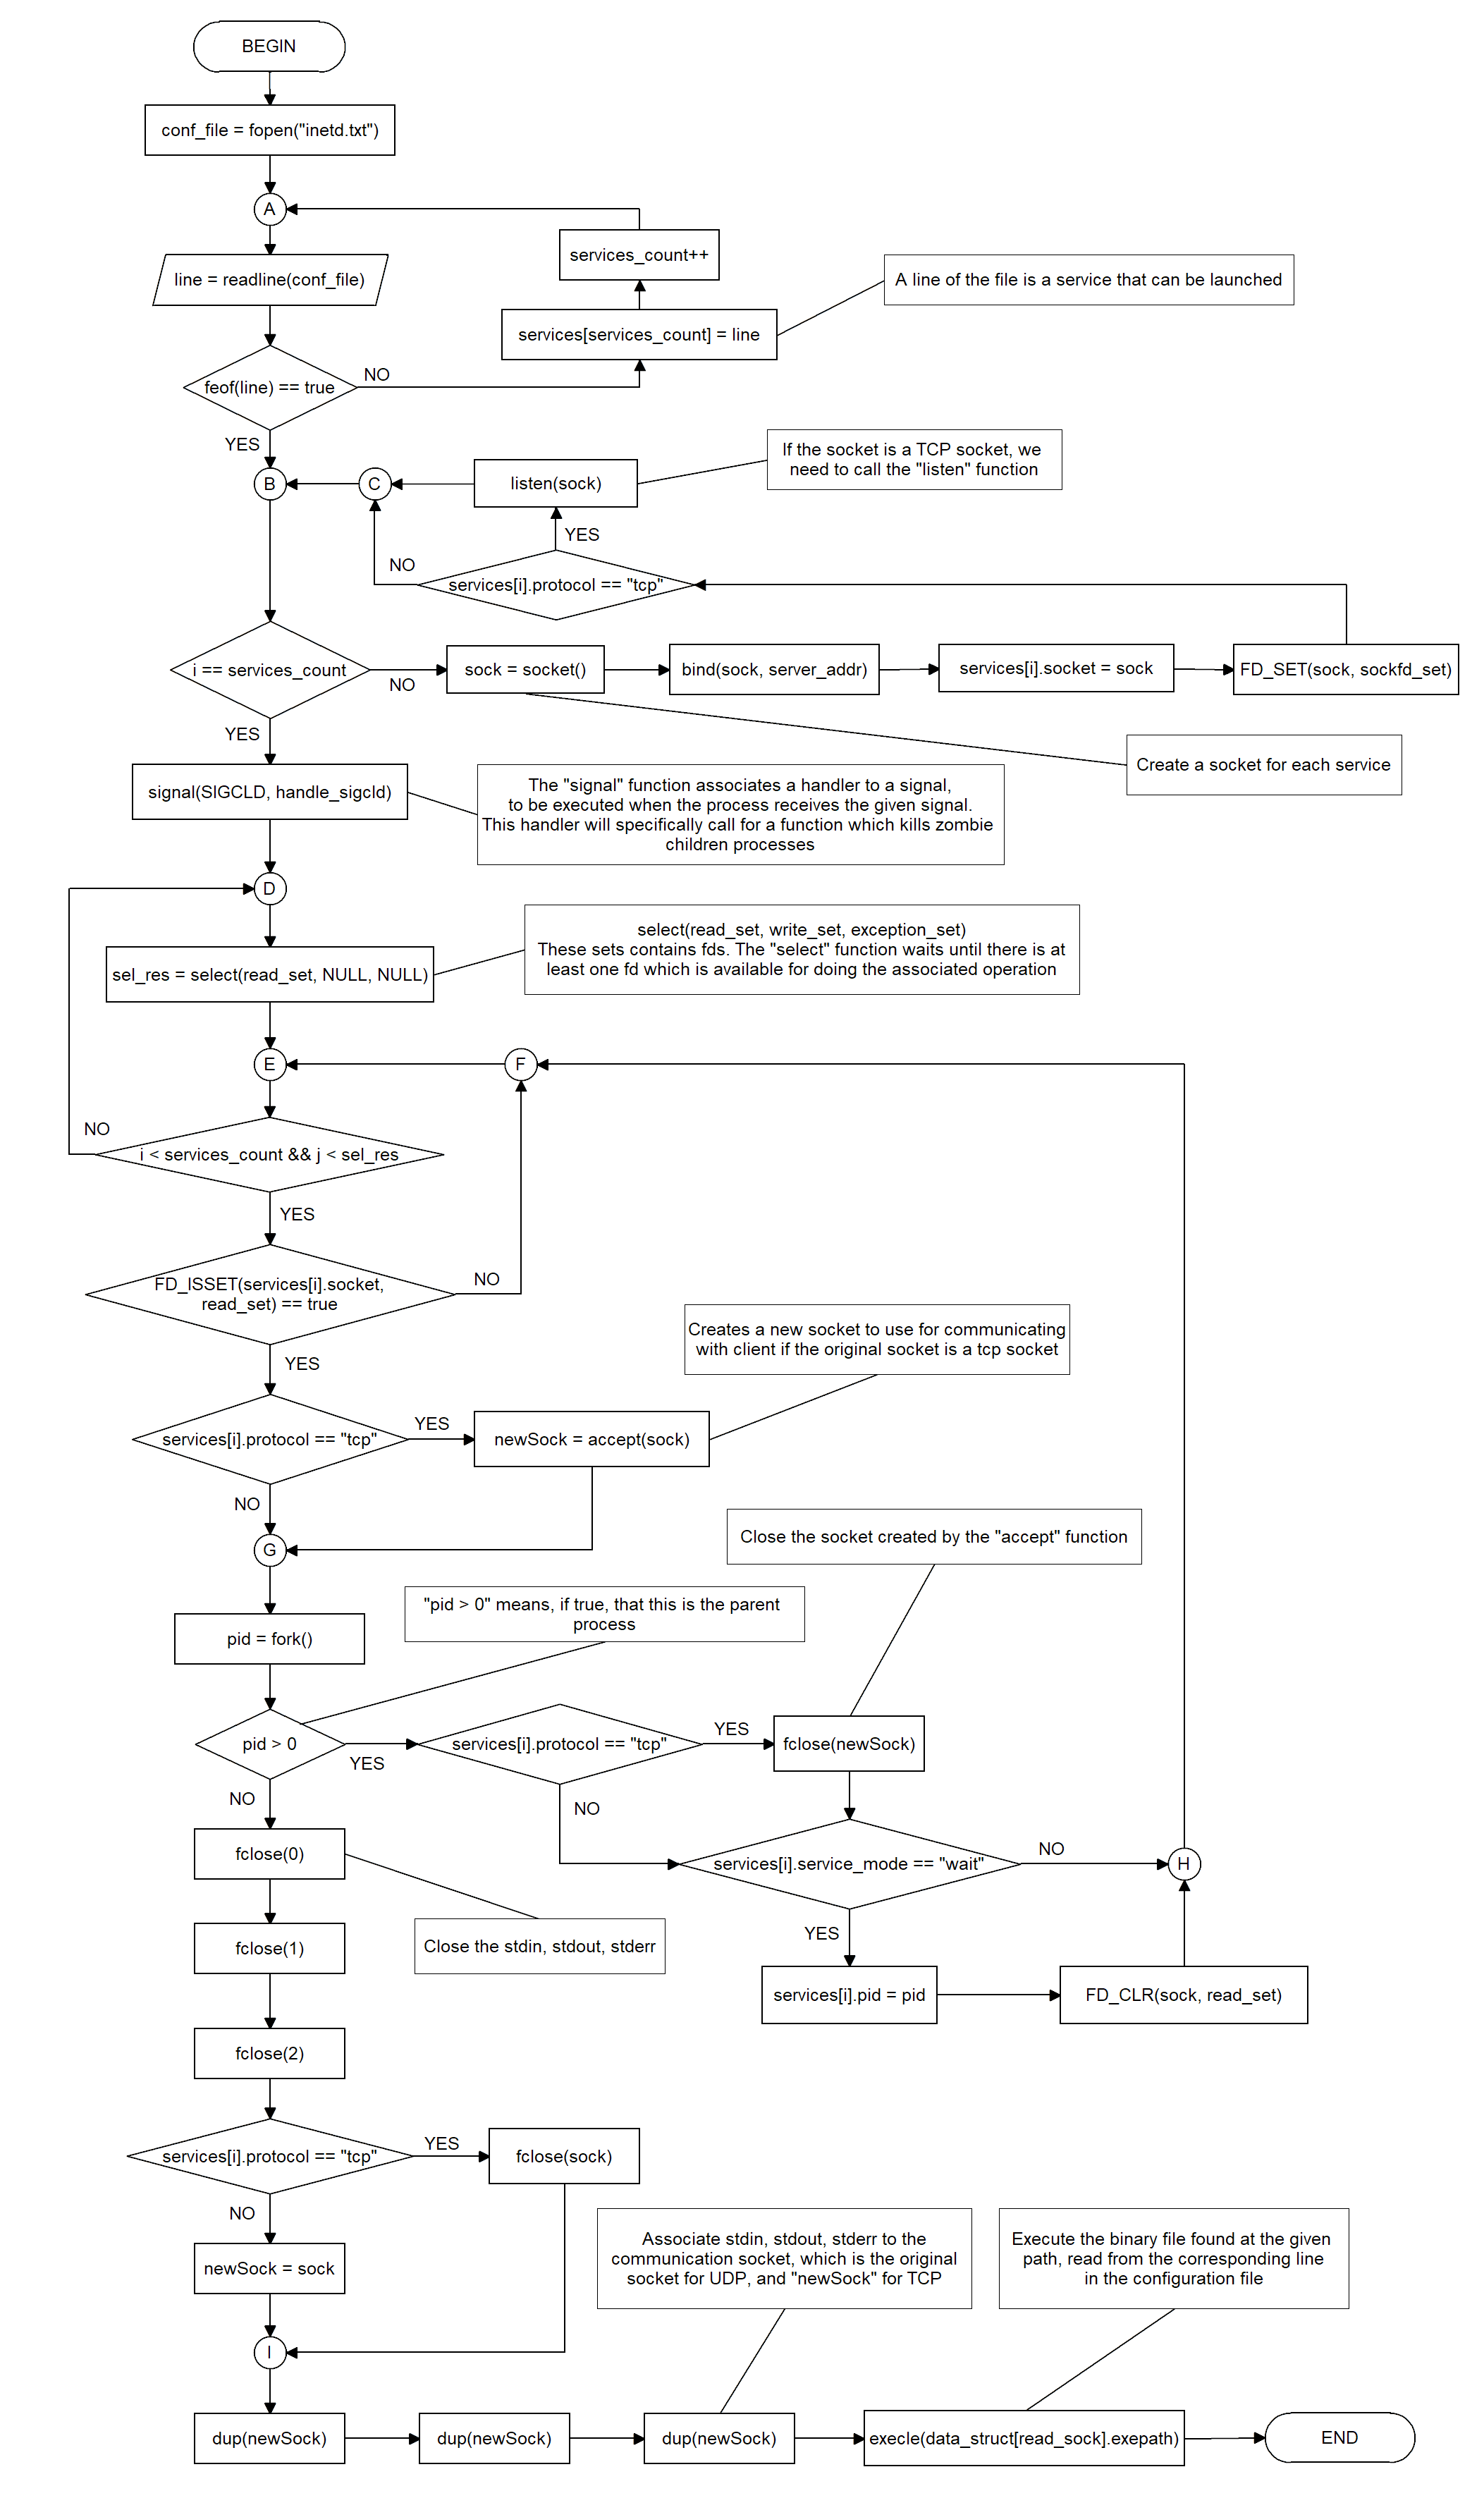
\includegraphics[width=\textwidth,height=\textheight,keepaspectratio]{images/diagram.png}
	\caption{Diagramma di flusso seguito nel programma scritto}
\end{figure}

Questo scherma rappresenta il flusso di controllo seguito dal programma, così come indicato nelle slide. Lo schema segue lo standard ISO 5807 per i diagrammi di flusso. Sono presenti
sotto forma di operazioni tutte le \textit{system call} utilizzate, nonchè le \textit{macro} per la gestione dei \textit{set} di \textit{file descriptor}. Per ciascuna delle prime è stato inserito
un commento che ne espliciti il funzionamento.

\chapter{Task Due}

\section{Design del \textit{superserver}}

\begin{itemize}
    \item Inizialmente viene definita la struttura dati sotto forma di ``struct" per ospitare tutte le informazioni necessarie per gestire un generico servizio
    \item Viene aperto il file ``inetd.txt" e viene letto riga per riga
    \item Ogni riga del file ha lo stesso formato di quattro parole: ``$<$percorso servizio$>$ $<$protocollo$>$ $<$porta$>$ $<$modalità servizio$>$". Queste informazioni vengono tutte
    memorizzate in una cella di un vettore di ``struct" definite come sopra. Si tiene traccia del numero di servizi salvati
    \item Viene inizializzato il \textit{set} dei ``\textit{socket file descriptor}" associati ai servizi salvati e viene creata una \textit{socket} per ogni servizio tramite le
    funzioni necessarie: ``socket", ``bind", anche ``listen" nel caso la socket fosse di associata al protocollo TCP. La \textit{socket}
    viene salvata assieme ai dati del servizio corrispondente nel vettore di ``struct" nonchè viene inserita nel \textit{set} indicato precedentemente
    \item Viene registrato l'\textit{handle} per il segnale di morte di un processo figlio, ``SIGCHLD". In questo modo, ogni volta che un processo figlio muore,
    se si occupava di gestire le richieste per un servizio in modalità ``wait", il \textit{superserver} si preoccupa di renderlo disponibile per i \textit{client} successivi che vogliono
    accedervi reinserendolo nel \textit{set} dei ``\textit{socket file descriptor}"
    \item La parte finale si basa su un ciclo che viene eseguito senza condizione di uscita, dove all'inzio si ha la funzione ``select". Questa permette al
    \textit{superserver} di rimanere in stato di \textit{wait} finchè almeno una socket è pronta per essere letta, ovvero un \textit{client} vuole comunicare con il
    \textit{superserver}. Si trova a sua volta in un ulteriore ciclo perchè alla presenza di un segnale mandato al processo che esegue il programma, si interrompe l'attesa della funzione mentre
    si vuole invece continuare ad attendere per i \textit{client}
    \item Allo scattare della ``select", per ogni \textit{socket} pronta, si controlla se è necessario usare la funzione ``accept" se essa è di tipo
    TCP. Dopodichè, si crea un processo figlio mediante la \textit{system call} ``fork"
    \item Il processo figlio è responsabile di chiudere ``stdin", ``stdout" e ``stderr" e sostituirli, mediante la \textit{system call} ``dup",
    con una \textit{socket}. Se il suo tipo è UDP, la \textit{socket} scelta per la sostituzione è quella nel vettore di ``struct", altrimenti se è di tipo TCP
    quella scelta è la \textit{socket} restituita dalla funzione ``accept", mentre quella nel vettore viene chiusa. Infine, il processo figlio sostituisce il proprio
    eseguibile binario con quello del servizio richiesto mediante la funzione ``execle"
    \item Nel frattempo, il processo padre, qualora la socket pronta fosse di tipo TCP, chiude la \textit{socket} per la comunicazione creata dalla funzione ``accept".
    In seguito, in caso il servizio richiesto fosse in modalità ``wait", rimuove dal \textit{set} dei ``\textit{socket file descriptor}" la socket appena entrata in
    uso. In questo modo, nessuno potrà più sfruttare quel servizio fino a che l'utilizzo da parte del \textit{client} corrente non sarà terminato. 
\end{itemize}

\section{Compilazione del \textit{superserver}}

È stato utilizzato il ``Makefile" incluso assieme agli altri \textit{file} di questo \textit{assignment}.

\section{Descrizione dei test effettuati per controllare il comportamento del \textit{superserver}}

Inizialmente sono stati compilati tutti i file sorgente, sia del \textit{superserver} sia quelli che ci sono stati forniti per ragioni di test.\newline
Sono stati posti nella stessa cartella dell'eseguibile del \textit{superserver} i file eseguibili ottenuti da ``tcpServer.c" e da ``udpServer.c", nonchè il file di
configurazione. Nel file di configurazione sono stati specificati quattro servizi, due con protocollo TCP - che sono l'eseguibile di ``tcpServer.c" - e due con protocollo UDP - che sono l'eseguibile di ``udpServer.c" -, ciascuno dei quali
ha come modalità specificata ``wait" oppure ``nowait" così da poter testare entrambi i protocolli in entrambe le modalità. È stato poi eseguito da terminale l'eseguibile
del \textit{superserver}. Per ciascuno dei quattro test, uno per servizio, sono stati eseguiti due processi \textit{client} come richiesto. Nel frattempo, in ciascuno
dei test, è stato tenuto aperto un terminale dove veniva eseguito il comando \textit{BASH} ``ps -aux" per visualizzare i processi correntemente in esecuzione ed osservare
quindi il numero di processi attivi dei \textit{server} avviati dal \textit{superserver} stesso.

\begin{figure}[H]
	\centering
	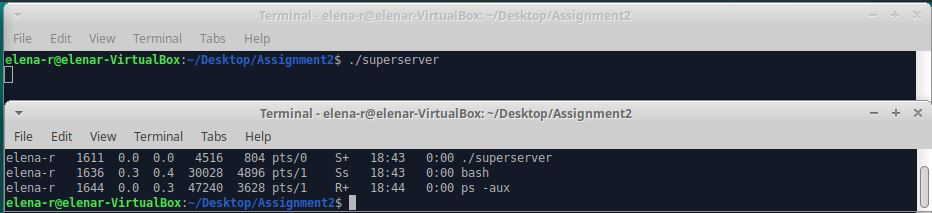
\includegraphics[width=\linewidth]{images/launch_superserver.JPG}
	\caption{Esecuzione dell'eseguibile del ``\textit{superserver}" nonchè del comando ``ps -aux"}
\end{figure}

Per ogni \textit{client}, l'indirizzo \textit{IP} passato come argomento all'esecuzione dello stesso è 
stato l'indirizzo di ``\textit{loopback}" 127.0.0.1, ricavato tramite il comando ``ifconfig". Il numero di porta passato come argomento all'esecuzione del processo \textit{client}
invece è stato scelto di volta in volta diverso tra i vari test, in modo da corrispondere alle indicazioni del file di configurazione ``inetd.txt".

\section{Comportamento del \textit{superserver}}

\begin{enumerate}
	\item Qual è il comportamento di ``udpServer"?
	\begin{itemize}
		\item Wait mode: è in esecuzione un solo ``udpServer", ma che è in grado di comunicare con entrambi i \textit{client} contemporaneamente. Questo perchè il protocollo UDP è
		\textit{connectionless} e ogni pacchetto che arriva fa vita a sè stante, cioè la \textit{socket} UDP non è identificata da informazioni come chi può mandare certi
		pacchetti a quella  \textit{socket}. Il fatto che sia presente una sola istanza del processo \textit{server} UDP è perchè il \textit{server} attende il completamento
		dell'operazione corrente prima di iniziarne una nuova tramite un nuovo processo, portandolo ad adempire le richieste di molteplici \textit{client} in modo sequenziale tramite
		un unico processo.
		\begin{figure}[H]
			\centering
			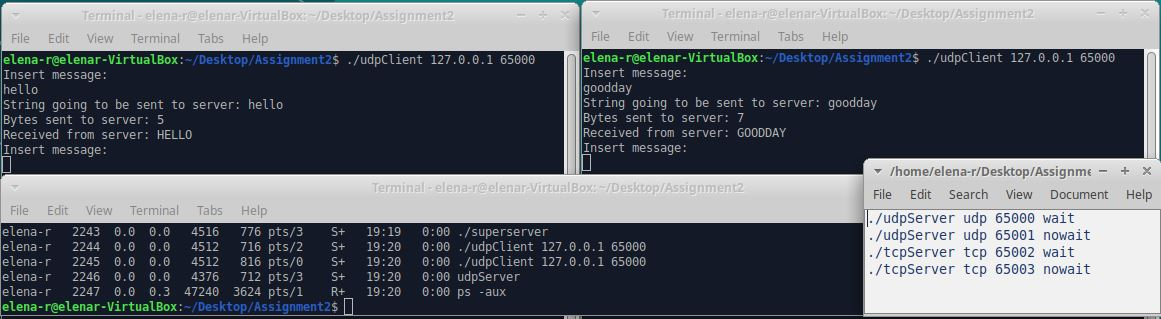
\includegraphics[width=\linewidth]{images/launch_udpClientWait.JPG}
			\caption{Test del \textit{server} UDP in modalità ``wait"}
		\end{figure}
		\item Nowait mode: in questo caso, l'unica differenza riscontrata è che se più di un \textit{client} si connette al \textit{server}, il \textit{server} crea molteplici processi al fine di
		soddisfare le richieste di ogni \textit{client} concorrentemente, così come indicato dal tipo di modalità, cioè ``nowait".
		\begin{figure}[H]
			\centering
			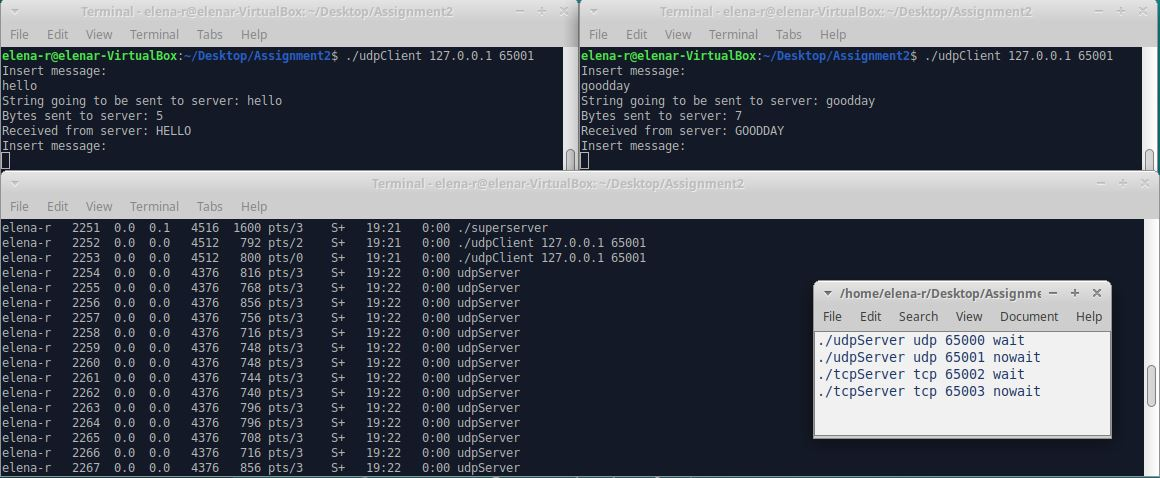
\includegraphics[width=\linewidth]{images/launch_udpClientNowait.JPG}
			\caption{Test del \textit{server} UDP in modalità ``nowait"}
		\end{figure}
	\end{itemize}
	\item Qual è il comportamento di ``tcpServer"?
	\begin{itemize}
		\item Wait mode: quando più \textit{client} tentano di connettersi al \textit{server}, esso interagisce con un solo \textit{client} alla volta; a differenza di UDP,
		poichè è \textit{connection-oriented}, il protocollo TCP necessita dell'instaurazione di una connessione con un \textit{client} per potervi comunicare.
		Il \textit{server} TCP perciò non può interagire con altri \textit{client} finché ha una connessione attiva perché attraverso essa riceve esclusivamente i pacchetti da uno
		specifico \textit{client} e nessun altro, al contrario di come avevamo visto per il \textit{server} UDP. Anche in questo caso, il \textit{server} TCP crea un solo
		processo e dopo la terminazione del primo processo \textit{client}, il \textit{server} si connette al secondo ed esegue le richieste di quest'ultimo e così via.
		\begin{figure}[H]
			\centering
			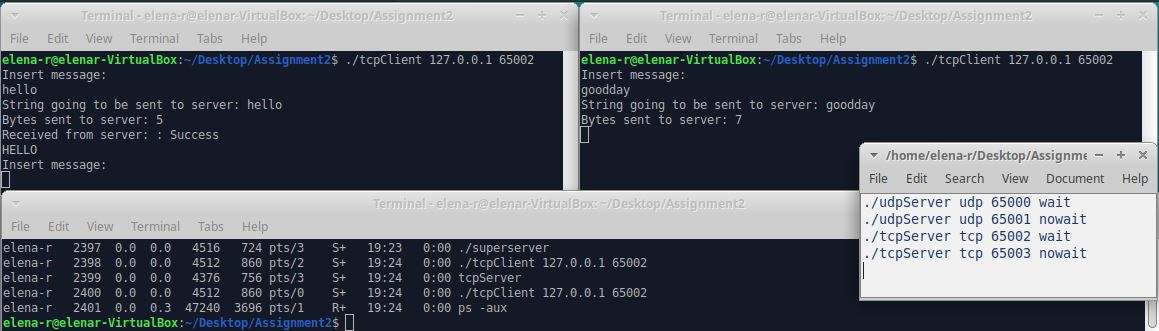
\includegraphics[width=\linewidth]{images/launch_tcpClientWait.JPG}
			\caption{Test del \textit{server} TCP in modalità ``wait" all'inizio}
		\end{figure}
		\begin{figure}[H]
			\centering
			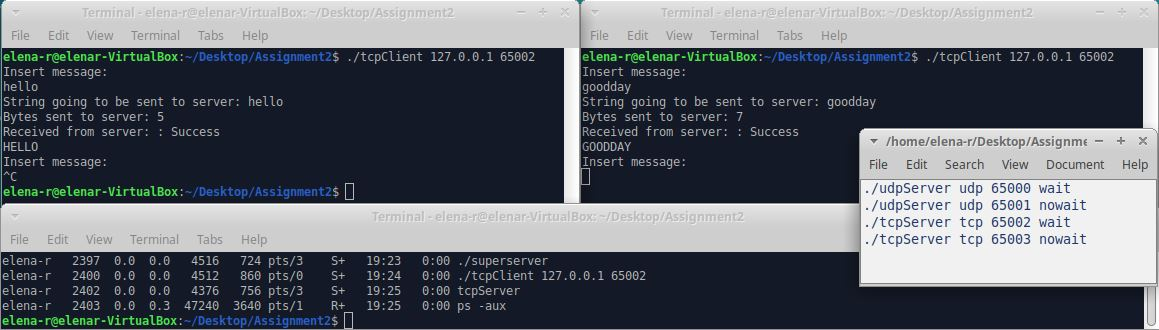
\includegraphics[width=\linewidth]{images/launch_tcpClientWait_2.JPG}
			\caption{Test del \textit{server} TCP in modalità ``wait" dopo la chiusura della connessione con il primo \textit{client}}
		\end{figure}
		\item Nowait mode: quando il \textit{server} TCP riceve molteplici richieste di connessione da parte di diversi \textit{client} crea un processo per ogni \textit{client}, così da
		poter interagire con essi contemporaneamente, in osservanza alla modalità concorrente scelta.
		\begin{figure}[H]
			\centering
			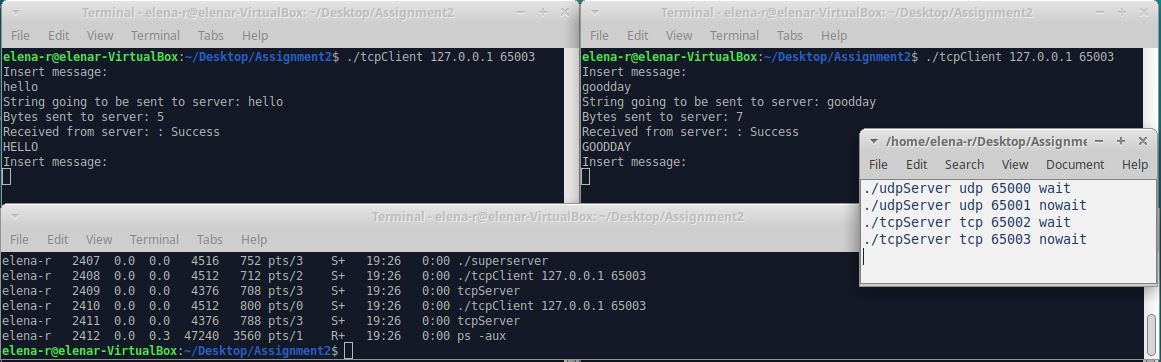
\includegraphics[width=\linewidth]{images/launch_tcpClientNowait.JPG}
			\caption{Test del \textit{server} TCP in modalità ``nowait"}
		\end{figure}
	\end{itemize}
\end{enumerate}

\end{document}
